\documentclass[10pt]{article}
\textwidth=7in
\textheight=9.5in
\topmargin=-1in
\headheight=0in
\headsep=.5in
\hoffset=-.85in
\pagestyle{empty}
\usepackage{amsmath}
\usepackage{tikz}
\usetikzlibrary{arrows}

\begin{document}

\begin{center}
{\bf CS165 Database Systems
\\ Homework 6 - Concurrency Control
\\ Solutions}
\end{center}

\noindent 1. A transaction $T_1$, executed by an airline reservation system, performs the following steps:

\begin{quote}
$i.$ It searches for flights and is able to load records $A$ and $B$ from the database. \\
$ii.$ Customer selects flight $B$ and a reservation is made for that customer. \\
$iii.$ Customer selects a seat for the flight, denoted by record $C$. \\
$iv.$ It fetches the customer's credit card data and sends a bill for the flight ($D$). \\
$v.$ Customer's rewards data and the flight's mileage are also loaded ($E$ and $F$). The customer's rewards data is then updated.
\end{quote}

\vskip.10in
\noindent {\bf Solution:} \\

\begin{quote}
$r_1(A);r_1(B);w_1(B);r_1(C);r_1(D);w_1(D);r_1(E);r_1(F);w_1(E)$
\end{quote}

\vskip.10in
\noindent 2. For the following schedule:

\begin{quote}
$r_1(A); r_2(A); r_3(B); w_1(A); r_2(C); r_2(B); w_2(B); w_1(C)$
\end{quote}

\vskip.10in
\noindent Answer the following questions:

\begin{quote}
$i.$ What is the precedence graph of the schedule? \\
$ii.$ Is the schedule conflict-serializable? If so, give one equivalent serial schedule.
\end{quote}

\vskip.10in
\noindent {\bf Solution:}

\vskip.10in
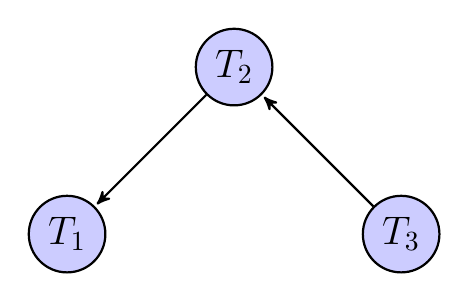
\begin{tikzpicture}[->,>=stealth',shorten >=1pt,auto,node distance=3cm,
  thick,main node/.style={circle,fill=blue!20,draw,font=\sffamily\Large\bfseries}]
\node[main node] (1) {$T_2$};
\node[main node] (2) [below left of=1] {$T_1$};
\node[main node] (3) [below right of=1] {$T_3$};
\path[every node/.style={font=\sffamily\small}]
	(1) edge node [right] {} (2)
	(3) edge node [right] {} (1);
\end{tikzpicture}

\vskip.10in
\noindent The schedule is conflict-serializable:

\begin{quote}
$r_1(A); r_2(A); r_3(B); w_1(A); r_2(C); r_2(B); w_2(B); w_1(C)$ \\
$r_2(A); r_1(A); r_3(B); w_1(A); r_2(C); r_2(B); w_2(B); w_1(C)$ \\
$r_2(A); r_1(A); w_1(A); r_3(B); r_2(C); r_2(B); w_2(B); w_1(C)$ \\
$r_2(A); r_1(A); w_1(A); r_2(C); r_3(B); r_2(B); w_2(B); w_1(C)$ \\
$r_2(A); r_1(A); r_2(C); w_1(A); r_3(B); r_2(B); w_2(B); w_1(C)$ \\
$r_2(A); r_2(C); r_1(A); w_1(A); r_3(B); r_2(B); w_2(B); w_1(C)$ \\
$r_2(A); r_2(C); r_1(A); w_1(A); r_2(B); r_3(B); w_2(B); w_1(C)$ \\
$r_2(A); r_2(C); r_1(A); w_1(A); r_2(B); r_3(B); w_2(B); w_1(C)$ \\
$r_2(A); r_2(C); r_1(A); r_2(B); w_1(A); r_3(B); w_2(B); w_1(C)$ \\
$r_2(A); r_2(C); r_2(B); r_1(A); w_1(A); r_3(B); w_2(B); w_1(C)$ \\
$r_2(A); r_2(C); r_2(B); r_1(A); w_1(A); w_2(B); r_3(B); w_1(C)$ \\
$r_2(A); r_2(C); r_2(B); r_1(A); w_2(B); w_1(A); r_3(B); w_1(C)$ \\
$r_2(A); r_2(C); r_2(B); w_2(B); r_1(A); w_1(A); r_3(B); w_1(C)$ \\
$r_2(A); r_2(C); r_2(B); w_2(B); r_1(A); w_1(A); w_1(C); r_3(B)$ \\
$r_3(B); r_2(A); r_2(C); r_2(B); w_2(B); r_1(A); w_1(A); w_1(C)$
\end{quote}

\vskip2.0in
\noindent 3. For the following schedule:

\begin{quote}
$r_1(A); r_2(B); r_3(C); w_1(B); w_2(C); w_3(D);$
\end{quote}

\vskip.10in
\noindent Insert shared and exclusive locks, and insert unlock actions. Place a shared lock ($sl_i(X)$) immediately in front of each read action that is not followed by a write action of the same element of the same transaction. Place an exclusive lock ($xl_i(X)$) in front of every other read or write action. Place the necessary unlocks at the end of every transaction.

\vskip.10in
\noindent {\bf Solution:}

\begin{quote}
$sl_1(A); r_1(A); sl_2(B); r_2(B); sl_3(C); r_3(C); ul_2(B); \\
xl_1(B); w_1(B); ul_3(C); xl_2(C); w_2(C); xl_3(D); w_3(D); \\
ul_1(A); ul_1(B); ul_2(C); ul_3(D)$
\end{quote}

\end{document}